%!TEX root = ../document.tex
\chapter{Buffer Overflow}
Buffer Overflow ist der Überbegriff für eine Schwachstelle im Quellcode der für einen Angriff genutzt wird und gehört zu den häufigsten Angriffsmethoden. Je nach Art der Schwachstelle wird auch von Heap-Overflow, Integer-Overflow oder String-Overflow gesprochen.

\section{Grundlegendes}
Einfach ausgedrückt, werden bei diesem Angriff einem Programm mehr Daten
übergeben als es erwartet bzw. verarbeiten kann. Bei guter Programmierung
führt dies zu einem Absturz des Programmes oder einer Fehlermeldung. Bei
schlechter Programmierung (fehlender Überprüfung der Eingangsdaten) reicht
der freigehaltene Speicherplatz für die Variable aber nicht aus und nachfolgende Speicherbereiche werden überschrieben.

Für das Überschreiben der nachfolgenden Speicherbereiche ist die Speicherverwaltung verantwortlich. Beim Start eines Programmes wird diesem nämlich ein bestimmter Speicherbereich zugewiesen. Dieser ist, wie in Abbildung \ref{fig:speicherAufbau} dargestellt, in drei Abschnitte aufgeteilt: den Code, den Heap und den Stack. Im Code liegt der eigentliche Quellcode, der nicht mehr verändert werden kann. Darüber liegt der Heap, in dem dynamische Variablen abgelegt sind. Der Stack beginnt am oberen Ende des Speichers und wächst mit jedem Eintrag nach unten. Dabei wird nach dem Prinzip des LIFO (last in, first out) vorgegangen. Gespeichert werden im Stack lokale Variablen, der Inhalt von Prozessorregistern und Rücksprung-Adressen von Unterprogrammen. Bei einem Angriff durch Buffer-Overflow wird einen lokale Variable mit mehr Daten beschrieben, als reserviert sind. Deshalb wird der nachfolgende Speicherbereich überschrieben, was entweder andere lokale Variablen oder aber Rücksprung-Adressen sein können.

Hier beginnt der eigentlich schädliche Angriff. Wurde zuvor bereits Schadcode auf dem Rechner des Opfers gespeichert, kann die Rücksprung-Adresse nun auf den Einsprungpunkt dieses Schadcodes zeigen. Mit Hilfe eines einfachen C-Programmes soll dies verdeutlicht werden. Darin wird zuerst ein Buffer angelegt und danach das beim Programmaufruf übergebene Argument in diesem Buffer gespeichert.
    \begin{figure}[H]
		\centering
		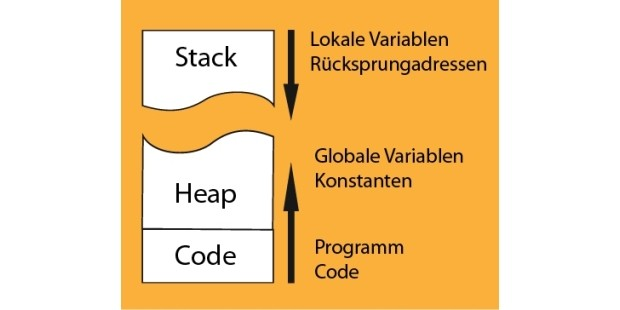
\includegraphics[width=1.0\textwidth]{images/bufferPics/speicherAufbau.jpg}
        \
		\caption{Aufbau des Speichers beim Start eines Programmes: Code -> Heap ->
Stack}
	\end{figure}
   		\label{fig:speicherAufbau}
        \begin{figure}[H]
		\centering
		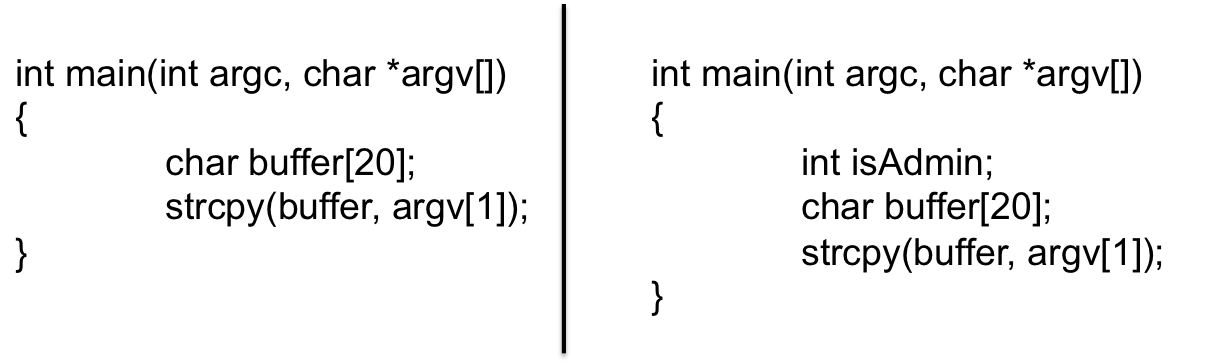
\includegraphics[width=1.0\textwidth]{images/bufferPics/beispielCode.png}        
		\caption{links: Eingabeargument wird nicht überprüft, kann aber keinen Schaden anrichten, rechts: Eingabeargument wird nicht überprüft und es ist möglich die Variable isAdmin zu überschreiben}
\label{fig:buffer1}
	\end{figure}
In Abbildung \ref{fig:buffer1} sind zwei kurze Programme nach diesem Aufbau gegeben.
Im linken Bild kann nicht viel passieren, da nur eine Variable gespeichert wird. Im
rechten Bild kann hingegen die Variable isAdmin bei zu langem Eingabeargument
überschrieben werden.
Um herauszufinden, ab wann es sich um eine „zu lange“ Eingabe handelt, muss
der Assembler Code des Programmes analysiert werden. Um herauszufinden wann es sich um eine zu lange Eingabevariable handelt, sollte der Stack, nach start des Testprogramms bufferOberflow.c, genauer betrachtet werden. Im diesen sind die Speicherreservierungen vorhanden. 
    \begin{figure}[H]
		\centering
		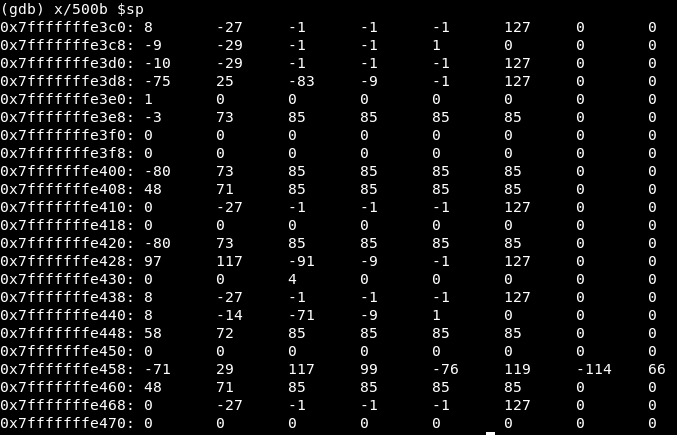
\includegraphics[width=1.0\textwidth]{images/bufferPics/Buffer1.png}
		\caption{Stackansicht mit dem noch nicht übergebenen Argument}
	\end{figure}
Jede Variable, die initialisert wurde, hat eine eindeutige Adresse. Kennt man die Adresse der Variablen, kann man sehen, welche Werte übergeben wurden. Somit ist zu sehen, wo eine Variable anfängt und die Andere aufhört. Dies macht man sich beim Buffer Overflow zu nütze. Es ist jedoch zu beachten, dass nach jedem Neuaufruf des C-Programmes, die Adressen der Variablen ändern sich könnten. Nichts desto trotz ist es sehr wahrscheinlich, dass die zuvor ermittelten Adressen, nach nochmaligen Programmaufruf, keine Veränderung aufwießen. 
Durch die Adressen der Variablen (Hex-Darstellung) kann man den Abstand zwischen diversen Variablen berechnen und daraus erschließen, wie viele Stellen bei dem Übergabeargument notwendig sind, um eine Speicherüberschreiben zu hervorrufen. 

\section{Vorbereitung}
Einen Raspberry Pi 3 Model b mit Kali 2.0, welcher als Angreifer oder Opfer vorgesehen ist und die aktuelle Security Workbench beinhält.

\section{Beispielaufgaben in der Security Workbench}
Das Tutorial besteht aus zwei einfachen Beispielen, bei denen ausgehend vom Quellcode eine Objekt-Datei erstellt und ausgewertet wird. Danach können selbstständig zwei weitere, ähnliche Aufgaben gelöst werden, bei denen lediglich die Objekt-Dateien vorhanden sind. Zur Durchführung dieses Tutorials muss lediglich die Security Workbench geöffnet und anschließend „Buffer Overflow“ mit Nummer "7" bestätigt werden. Beide Beispiele sind so konzipiert, dass der Anwender durch das Beispiel geführt wird. Es wird genau beschrieben, welche Eingabe getätigt werden müssen, um zum nächsten Schritt weiter zu kommen. 

\subsection{Erstes Beispiel}
Um das erste Beispiel zu starten, wähle beim ersten Durchgang des Tutorials, die Nummer 1 „Erstes Beispiel“.
Daraufhin soll der Quellcode in ein ausführbares Programm kompiliert werden.\\ \textbf{Dies wird mit folgendem Befehl gemacht:}\\\\
\bashCommand{gcc -ggdb BufferOverflow / FirstExample .c -o BufferOverflow / FirstExample}\\\\
(\bashCommand{gcc} startet den GNU Kompiler und speichert aufgrund der Option \bashCommand{-ggdb <name>} auch Informationen des angegebenen Programmes, die später mit dem GNU Debugger ausgelesen werden können, mit \bashCommand{-o <name>} wird außerdem der Name angegeben unter dem die erstellte Objekt-Datei gespeichert werden soll)\\\\
Der Anwender sollte sich daraufhin mit dem C-Programm vertraut machen, ein eigenes Consolenfenster erscheint und es wird der genannte C-Code angezeigt.\\ \textbf{Der Befehl dazu ist:}\\\\
\bashCommand{view BufferOverflow/FirstExample.c}\\\\
Der Quellcode von BufferOverflow/FirstExample.c kann nun genauer analysiert werden. Es ist auffallend, dass darin zuerst zwei Variablen angelegt werden.
Im Anschluss wird das Eingabeargument in die Array-Variable "buffer[8]" gespeichert. Da das Argument vor der Speicherung nicht auf seine Größe überprüft wird, ist es möglich weitere Variablen, mit einer zu großen Eingabe, zu überschreiben.
Im Zusammenhang dazu, sollten nun die wichtigen Variablen "buffer[]" und "authflag" gemerkt werden. Da diese wichtig sind für das Verständnis des 1. Beispiels. Anschließend kann das Consolenfenster wieder geschlossen werden.\\
Nach bestätigen des vorherhigen Schrittes mit Enter, wird nun Zeit den Assembler-Code, des erzeugten Programmes, mit dem GNU Debugger zu analysieren. Da hier ein Unterprozess geöffnet wird, startet ein neues Terminal mit dem GNU Debugger. Wie dieses aussieht, kann man in Abbildung 10.3 sehen. Es wird empfohlen im ersten Terminal weiter die Befehle durchzugehen und im Zweiten, den Assembler-Code zu analysieren. 
\\
\textbf{Gestartet wird der GNU Debugger mit dem Befehl:}\\\\
\bashCommand{gdb BufferOverflow / FirstExample}\\\\
Der nächste folgende Schritt ist, dass ein breakpoint bei Line 10 gesetzt wird. Die Zeile 10 ist deshalb gewählt worden, da noch nicht das Übergabeargument im Stack übergeben wurde. Der Benutzer hat somit die Möglichkeit den Stack vorher und nachher anzuschauuen und die Veränderungen leichter zu erkennen. Den Breakpoint wird mit\\\\ \bashCommand{break 10}\\\\ gesetzt. Nach diesem Befehl sollte der User\\\\ \bashCommand{x/500b \$sp}\\\\ eingeben. 
\\
Mit "q" kann man die Stackansicht verlassen. Es ist erstmal nur der Aufbau mit diversen Adressen und Dezimalwerten von FirstExample.c erkennbar. Interessant sind jedoch nur die Adressen von buffer und authflag. Um die Adressen aber anzeigen zu lassen, muss erst das Programm mit Übergabeargument gestartet werden. Dies wird z.B. folgend ermöglicht:\\\\\bashCommand{run AAAAAA}\\\\Daraufhin kann man die Adressinformation mit folgenden Befehl anzeigen lassen:\\\\ \bashCommand{print buffer}\\ \bashCommand{print authflag}\\\\Es ist sind die beiden Adressen in Hex-Darstellung zu sehen. Der Benutzer weiß nun wo er genauer hinschauen muss und wo er das Eingabeargument erwarten wird. Mit\\\\ \bashCommand{next}\\\\wird das Programm um eine Zeile fortgesetzt. Das Übergabeargument sollte also übergeben sein, deshalb wird die Stackansicht nochmal aufgerufen. Es ist zu erkennen, dass beginnend bei der Startadresse von buffer[] der Wert 65 steht. Die Zahl 65 ist der Dezimmalwert des Buchstaben A, welcher mehrfach als Übergabeargument übergeben wurde. Um nun einen Buffer Overflow herbeizuführen, muss man z.B. genügend viele A's übergeben bis die Adresse von authflag überschrieben wurde. Der Anwender hat zwei möglichkeiten um herauszufinden wie lang sein Argument sein soll. Er kann zählen wie viele Stellen er benötigt, bis zu der Adresse "authflag" oder er subtrahiert die beiden Hex-Adressen und stellt das Ergebnis als Dezimalwert da. Hat der Anwender die benötigte Anzahl ermittelt, kann das zweite Consolenfenster des GNU Debugger mit\\\\ \bashCommand{quit}\\\\beendet werden. Nachfolgend wird der Benutzer in der Menüführung aufgefordert nochmals das Programm starten mit einem nicht ausreichender Länge des Übergabearguments. Als Antwort wird ein Zugriff verwehrt ausgegeben. Daraufhin soll nun ein Übergabeargument gewählt werden, was zu einem überschreiben der Variable "authflag" fühen würde. Ist das Argument ausreichend lang gewählt worden. Werden die Kontoinformation von Max Mustermann ausgegeben.\\\\Ein Beispiel:\\\\Starte nun das ausfuehrbare Programm FirstExample aus dem Unterordner BufferOverflow und gib als Eingabewert einen String mit so vielen Stellen mit, dass die Daten eines Bankkunden noch nicht mit ausgegeben werden.\\\\
\bashCommand{./BufferOverflow/FirstExample AAAAA}\\
\textbf{Ausgabetext:} Ungueltige Eingabe! -> Zugriff verweigert!
\\\\
Starte nun das ausfuehrbare Programm FirstExample aus dem Unterordner BufferOverflow und gib als Eingabewert einen String mit so vielen Stellen mit, dass die Daten eines Bankkunden mit ausgegeben werden.\\\\
\bashCommand{./BufferOverflow/FirstExample AAAAAAAAAAAAAAAAAAAAAAAAAAAAAAAAAAAAAAAAAAAAAAAAAAAA}\\
(Abhängig von der ermittelten Länger der Adressen)\\\\
\textbf{Ausgabetext:} Zugriff gewaehrt! Die Kontodaten von Max Mustermann sind: DE123456678
\\
\subsection{Zweites Beispiel}
Um das zweite Beispiel zu starten, wähle beim ersten Durchgang des Tutorials, die Nummer 2 „Zweites Beispiel“.
Daraufhin soll der Quellcode in ein ausführbares Programm kompiliert werden.\\ \textbf{Dies wird mit folgendem Befehl gemacht:}\\\\
\bashCommand{gcc -ggdb BufferOverflow / SecondExample .c -o BufferOverflow / SecondExample}\\\\
(\bashCommand{gcc} startet den GNU Kompiler und speichert aufgrund der Option \bashCommand{-ggdb <name>} auch Informationen des angegebenen Programmes, die später mit dem GNU Debugger ausgelesen werden können, mit \bashCommand{-o <name>} wird außerdem der Name angegeben unter dem die erstellte Objekt-Datei gespeichert werden soll)\\\\
Der Anwender sollte sich daraufhin mit dem C-Programm vertraut machen, ein eigenes Consolenfenster erscheint und es wird der genannte C-Code angezeigt.\\ \textbf{Der Befehl dazu ist:}\\
\bashCommand{view BufferOverflow/SecondExample.c}\\\\
Der Quellcode von BufferOverflow/SecondExample.c kann nun genauer analysiert werden. Es ist auffallend, dass darin zuerst drei Variablen angelegt werden.
Im Anschluss wird das Eingabeargument in die Array-Variable 'buffer[8]' gespeichert. Da das Argument vor der Speicherung nicht auf seine Größe überprüft wird, ist es möglich weitere Variablen, mit einer zu großen Eingabe, zu überschreiben.
Im Zusammenhang dazu, sollten nun die wichtigen Variablen 'buffer[]', 'authflag' und die neue Variable 'checkForHack' gemerkt werden. Da diese wichtig sind für das Verständnis des zweiten Beispiels. Die Besonderheit des zweiten Beispiels ist, dass checkForHack bei Veränderung des Wertes nicht mehr die Adminrechte gewährleistet. Es ist also notwendig, die Variable unberührt oder denselben Wert an diese zu übergeben. Anschließend kann das Consolenfenster wieder geschlossen werden.
Nach bestätigen des vorherhigen Schrittes mit Enter, wird nun Zeit den Assembler-Code, des erzeugten Programmes, mit dem GNU Debugger zu analysieren. Da hier ein Unterprozess geöffnet wird, startet ein neues Terminal mit dem GNU Debugger. Wie dieses aussieht, kann man in Abbildung 10.3 sehen. Es wird empfohlen im ersten Terminal weiter die Befehle durchzugehen und im Zweiten, den Assembler-Code zu analysieren. 

\textbf{Gestartet wird der GNU Debugger mit dem Befehl:}\\\\
\bashCommand{gdb BufferOverflow / SecondExample}\\\\
Der nächste folgende Schritt ist, dass ein breakpoint bei Line 10 gesetzt wird. Zeile 10 ist deshalb gewählt worden, da noch nicht das Übergabeargument im Stack übergeben wurde. Der Benutzer hat somit die Möglichkeit den Stack vorher und nachher anzuschauen und die Veränderungen leichter zu erkennen. Den Breakpoint wird mit\\\\ \bashCommand{break 10}\\\\ gesetzt. Nach diesem Befehl sollte der User\\\\ \bashCommand{x/500b sp}\\\\ eingeben. 
%TODO dollarzeichen!!!
%TODO verweis auf buffer1
Mit "q" kann man die Stackansicht verlassen. Es ist erstmal nur der Aufbau mit diversen Adressen und Dezimalwerten von FirstExample.c erkennbar. Interessant sind jedoch nur die Adressen von buffer,authflag und checkForHack. Um die Adressen aber anzeigen zu lassen, muss erst das Programm mit Übergabeargument gestartet werden. Dies wird z.B. folgend ermöglicht:\\\\\bashCommand{run AAAAAA}\\\\Daraufhin kann man die Adressinformation mit folgenden Befehl anzeigen lassen:\\\\ \bashCommand{print buffer}\\ \bashCommand{print checkForHack}\\ \bashCommand{print authflag}\\\\Es ist sind die drei Adressen in Hex-Darstellung zu sehen. Der Benutzer weiß nun wo er genauer hinschauen muss und wo er das Eingabeargument erwarten wird. Es fällt jedoch auf, dass die Variable checkForHack vom Adressbereich zwischen buffer und authflag liegt. Hierzu in Kürze mehr. Mit\\\\ \bashCommand{next}\\\\wird das Programm um eine Zeile fortgesetzt. Das Übergabeargument sollte also übergeben sein, deshalb wird die Stackansicht nochmal aufgerufen. Es ist zu erkennen, dass beginnend bei der Startadresse von buffer[] der Wert 65 steht. Die Zahl 65 ist der Dezimmalwert des Buchstaben A, welcher mehrfach als Übergabeargument übergeben wurde. Um nun einen Buffer Overflow herbeizuführen, muss man z.B. genügend viele A's übergeben bis die Adresse von authflag überschrieben wurde. Der Anwender hat zwei möglichkeiten um herauszufinden wie lang sein Argument sein soll. Er kann zählen wie viele Stellen er benötigt, bis zu der Adresse "authflag" oder er subtrahiert die beiden Hex-Adressen und stellt das Ergebnis als Dezimalwert da. Genau hier liegt das Problem, denn ein entsprechend langes Übergabeargument überschreibt nicht nur die Variable authflag sondern auch die Variable checkForHack. Das Überschreiben von checkForHack, welches zu einem anderen Wert führen könnte, sollte jedoch vermieden werden. Bei genaurer Analyse dieser Variable fällt auf, dass der Wert im SecondExample.c den Wert -559038737 (dec) aufweist bzw. erwrtet. Dieser Wert entspricht den Hex-Wert von 0x DEAD BEEF.\\\\ \textbf{Aufgeteilt:} 
\begin{itemize}
\item 0xDE
\item 0xAD
\item 0xBE
\item 0xEF
\end{itemize}
Da der Stack jedoch von unten nach oben schreibt, ist es notwendig das in umgekehrter Reihenfolge die Hex-Werte betrachtet werden müssen.
\begin{itemize}
\item 0xEF
\item 0xBE
\item 0xAD
\item 0xDE
\end{itemize}
Das Programm interpretiert die Eingabe mit Unicode über Codepage 850. Das heißt, dass jeder Unicode ein eigenes Zeichen entspricht und dieses Zeichen an richtiger Stelle im Übergabeargument eingetragen werden muss. Damit wird authflag überschrieben und die Variable checkForHack wird der gleiche Wert wie voher übergeben und somit kann das Lösungswort bzw. die Bankdaten von Max Mustermann ausgeben werden.\\\\\textbf{Im folgenden wird aufgezeigt, welches Zeichen welcher Unicode entspricht:}
\begin{itemize}
\item EF = ï
\item BE = ¾
\item AD = -
\item DE = Þ
\end{itemize}

Hat der Anwender die benötigte Anzahl ermittelt, kann das zweite Consolenfenster des GNU Debugger mit\\\\ \bashCommand{quit}\\\\beendet werden. Nachfolgend wird der Benutzer in der Menüführung aufgefordert nochmals das Programm zu starten mit einem nicht ausreichender Länge des Übergabearguments. Als Antwort wird eine Zugriffsverweigerung ausgegeben. Daraufhin soll nun ein Übergabeargument gewählt werden, welche zu einem überschreiben der Variable "authflag" führen würde. Ist das Argument ausreichend lang gewählt, werden die Kontoinformation dennoch nicht, wie beim Ersten Beispiels, von Max Mustermann ausgegeben. Grund dafür ist das Überschreiben der Variable checkForHack.\\\\Ein Beispiel:\\\\Starte nun das ausfuehrbare Programm FirstExample aus dem Unterordner BufferOverflow und gib als Eingabewert einen String mit so vielen Stellen mit, dass die Daten eines Bankkunden noch nicht mit ausgegeben werden.\\\\
\bashCommand{./BufferOverflow/SecondExample AAAAA}\\
\textbf{Ausgabetext:} Ungueltige Eingabe! -> Zugriff verweigert!
\\\\
Starte nun das ausfuehrbare Programm SecondExample aus dem Unterordner BufferOverflow und gib als Eingabewert einen String mit so vielen Stellen mit, dass die Daten eines Bankkunden mit ausgegeben werden.\\\\
\bashCommand{./BufferOverflow/SecondExample AAAAAAAAAAAAAAAAAAAAAAAAAAAAAAAAAAAAAAAAAAAAAAAAAAAA}\\
(Abhängig von der ermittelten Länger der Adressen)\\\\
\textbf{Ausgabetext:} Ungueltige Eingabe! -> Zugriff verweigert!
\\\\
\textbf{Richtig wäre hier gewesen:}\\\\
\bashCommand{./BufferOverflow/SecondExample AAAAAAAAAAAAAAAAAAAAAAï¾-ÞAAAAAAAAAAAAAAAAAAAAAA}
\\\\
Hier wurde an die Adresse von checkForHack der gleiche Wert übergeben, welcher von dem C-Programm vorrausgesetzt wurde. Deshalb wäre die Ausgabe wie folgend.\\
\textbf{Ausgabetext:} Zugriff gewaehrt! Die Kontodaten von Max Mustermann sind: DE123456678

\subsection{Aufgaben}
Zusätzlich zu den beiden gerade erklärten Beispielen stehen zwei Aufgaben zur Verfügung. Bei diesen ist lediglich die Objekt-Datei gegeben und es soll auch hier herausgefunden werden, wie viele Stellen das Eingabeargument besitzen muss, damit das Passwort  usgegeben wird (weil man die Administratorvariable
überschrieben hat).
Die Aufgaben liegen im Unterordner Projekte/BufferOverflow und heißen Buffer1 bzw. Buffer2.

\section{Gegenmaßnahmen}

\subsection{Programmierer}
Ist man selbst der Programmierer und möchte Angriffe auf den eigenen Code verhindern, ist die einfachste Methode das Benutzen von modernen Compilern in Kombination mit Visual C++ 2010-Projekten.
Diese prüfen bereits beim Compilieren, ob etwa unsichere Befehle wie strcpy anstatt der sicheren Variante von strcpy\_s verwendet werden und gibt entsprechende Warnungen aus. 
Sollte diese Warnung ignoriert werden, so wird trotzdem ein sicherer Code erzeugt, da automatische Funktionen in den Code mit eingepflegt werden. 
Zu diesen Funktionen gehört die Adress space layout randomization (ASLR) die der Funktion bei jedem Programmstart eine neue Adresse im Speicher zuweist. 
Der Compiler-Schalter/GS ist eine Puffersicherheitsüberprüfung, die einen Buffer Overflow abfängt und das Programm aufgrund des Compiler-Schalters /RTC1 (zur vollständigen Laufzeitüberprüfung) die Programmausführung abbricht. 
Dass trotz all diesen Möglichkeiten noch Buffer Overflow-Angriffe möglich sind, liegt an den alten Entwicklungsumgebungen. 
Viele Programme werden noch in solchen erstellt, da das Umziehen von Software auf neuer Umgebungen sehr viel Aufwand benötigt. 
Außerdem haben Hacker mittlerweile auch Methoden gefunden, um diese Sicherungen zu umgehen.

\subsection{Benutzer}

Als Benutzer eines Programmes ist man darauf angewiesen, dass der Hersteller seine Programme möglichst gut abgesichert hat. Durch regelmäßige Updates kann man den neuesten Schutz des Herstellers verwenden.
Eine andere Möglichkeit ist die Wahl von alternativer Software (Foxit Reader statt Adobe Reader). Hier kann man auf wenig Hacker-Angriffe hoffen, da diese normalerweise für einen großen Effekt weit verbreitete Software angreifen.
Die letzte Möglichkeit stellt das kostenloses Microsoft Tool Emet (Enhanced Mitigation Experience Toolkit) dar. Dieses sichert Programme nachträglich mit den im vorherigen Abschnitt erklärten Schutzmechanismen ab und bietet somit zumindest einen kleinen Schutz vor Angriffen.